%% =====================================================================
%% PACER: Perturbation-Aware Contrastive Framework for Long-Tail
%%        Multimodal Recommendation --- single-axis architectural design
%% KSE 2026 --- IEEE conference template --- v14
%% Rev14 (over v13) --- honest 5-seed re-report and 250-ep RQ4:
%%   * RQ2 (Sec.V-C, Table III): the v13 "20-epoch smoke test on
%%     seed 42" paragraph and its +0.759 pp claim are replaced by the
%%     real 5-seed 100-epoch NRDMC-lite ablation. A0 beats A1 by
%%     +0.114 pp R@20 (paired-t df=4 p=0.117, d_z=+0.89, dir 4/5),
%%     +0.083 pp N@20 (p=0.029, d_z=+1.48, dir 5/5), and
%%     +0.006 pp P@20 (p=0.113, d_z=+0.90, dir 4/5). We now
%%     explicitly frame R@20 as directional-large-effect but
%%     power-limited at n=5.
%%   * RQ4 (Sec.V-E, Table V): added a second PACER row for the
%%     250-epoch "PACER-full-new" configuration. Head recedes
%%     to 0.1527 (+11.9%%), Mid rises to 0.0452 (+104.4%%), Tail rises
%%     to 0.0204 (+128.9%%), overall Recall@20 unchanged (10.39 vs
%%     10.39 at 100-ep). This documents that at convergence
%%     NRDMC-lite reallocates capacity from Head to Mid/Tail at
%%     constant overall R@20 (paired-t p<0.05 on all three
%%     tercile contrasts vs 100-ep A0).
%%   * RQ5 (Sec.V-F, Table VI): B10 promoted from n=2 to n=5
%%     (10.377+/-0.058); statistical readout rewritten with the
%%     three most informative two-sided paired-t (df=4) contrasts
%%     (B11 vs B00 p=0.040, B11 vs B10 p=0.074, B11 vs B01 p=0.82);
%%     the erroneous v13 p=0.003 for B11 vs B00 is corrected.
%%   * Conclusion updated to reflect the honest RQ2 framing.
%% All other structure (v13 TAMER-lineage Fig 1, Sec.IV-D adopted/
%% modified/dropped table, Related Work TAMER paragraph, RQ1 shipping
%% cell) is preserved unchanged.
%% First author:  Minh-Khoi Le            khoilm@vnu.edu.vn
%% Second author: Duc-Trong Le (corresponding)  trongld@vnu.edu.vn
%% VNU University of Engineering and Technology, Hanoi, Vietnam
%% =====================================================================
\documentclass[conference]{IEEEtran}
\IEEEoverridecommandlockouts

% ===================== Encoding =====================
\usepackage[utf8]{inputenc}
\usepackage[T1]{fontenc}
\usepackage[english]{babel}
\DeclareFontShape{T1}{ptm}{m}{scit}{<->ssub*ptm/m/it}{}

% ===================== Math =====================
\usepackage{amsmath,amssymb,amsfonts,amsthm}
\usepackage{mathtools}
\usepackage{bm}

% ===================== Graphics & Diagrams =====================
\usepackage{graphicx}
\usepackage{tikz}
\usepackage{pgfplots}
\pgfplotsset{compat=1.18}
\usetikzlibrary{
  arrows.meta, calc, positioning, shapes.geometric, shapes.misc,
  fit, backgrounds, decorations.pathreplacing, decorations.markings,
  patterns, matrix, chains, scopes
}

% ===================== Tables & Misc =====================
\usepackage{booktabs}
\usepackage{multirow}
\usepackage{array}
\usepackage{enumitem}
\usepackage{xcolor}
\usepackage{cite}

% ===================== Colours for diagrams =====================
\definecolor{accentteal}{HTML}{20808D}
\definecolor{accentdark}{HTML}{1B474D}
\definecolor{accentterra}{HTML}{A84B2F}
\definecolor{accentgold}{HTML}{D19900}
\definecolor{accentcyan}{HTML}{BCE2E7}
\definecolor{accentolive}{HTML}{848456}
\definecolor{accentmauve}{HTML}{944454}
\definecolor{bgsoft}{HTML}{F7F6F2}
\definecolor{passgreen}{HTML}{437A22}
\definecolor{negativered}{HTML}{A13544}
\definecolor{accentblue}{HTML}{006494}

% ===================== Shortcuts =====================
\newcommand{\Lcal}{\mathcal{L}}
\newcommand{\Ucal}{\mathcal{U}}
\newcommand{\Ical}{\mathcal{I}}
\newcommand{\Ecal}{\mathcal{E}}
\newcommand{\norm}[1]{\left\lVert #1 \right\rVert}
\newcommand{\inner}[2]{\langle #1,\, #2 \rangle}
\newcommand{\sg}{\mathrm{sg}}
\newcommand{\tbd}{{\normalfont\itshape\textcolor{gray}{pending}}}

% ===================== Metadata =====================
\title{PACER: A Perturbation-Aware Contrastive Framework\\for Long-Tail Multimodal Recommendation}

\author{
\IEEEauthorblockN{Minh-Khoi Le, Duc-Trong Le$^{*}$}
\IEEEauthorblockA{VNU University of Engineering and Technology, Hanoi, Vietnam\\
\{khoilm, trongld\}@vnu.edu.vn}
\thanks{$^{*}$Corresponding author.}
}

\begin{document}
\maketitle

% =====================================================================
\begin{abstract}
Modern multimodal recommenders combine graph propagation with an
InfoNCE contrastive head. A recurring failure mode is that raw
ResNet-50 and Sentence-BERT features carry sensor and semantic noise
which, once propagated through LightGCN, disproportionately harms
long-tail items whose small neighbourhoods offer weak averaging. We
propose \textbf{PACER}, a \emph{perturbation-aware contrastive
framework} whose single architectural contribution is
\textbf{NRDMC-lite}, a parameter-efficient view-contrastive denoiser
that learns a semantic-aware view (SAV) and an interest-aware view
(IAV) over the observed user--item graph, adaptively fuses their edge
weights, propagates the resulting weighted graph for $K{=}2$ LightGCN
steps, and pulls the trunk representation toward the view embedding
through a batch-N InfoNCE loss. NRDMC-lite adds only $d{+}2$ learnable
parameters ($d{=}128$; $130$ parameters absolute) and composes with
any LightGCN-style backbone. On Amazon Clothing, over the five
KSE-locked seeds, PACER lifts an in-house MMHCL reproduction from
$8.737$ to $10.407$ Recall@20 ($+19.12\%$; paired-$t$ $p<10^{-4}$),
driven primarily by a Mid-tercile gain of $+89.5\%$ and a Tail-tercile
gain of $+98.4\%$. PACER's encoder-side preprocessing (multi-component whitening of the
text modality, PCA$\to$ICA and ZCA streams) and its interest-tree
augmented item-item cache both derive from TAMER~\cite{meng2025tamer};
Section~\ref{sec:tamerrel} makes the reuse explicit and states which
TAMER components we adopt verbatim, which we modify, and which we
drop. We additionally report a \emph{systematic component analysis}
that stress-tests two auxiliary design axes---a TAMER-style
interest-tree cache with an RSFPGrowth-blended item-item source and a
Log$Q$-Laplace popularity debias---and find them both statistically
neutral or negative on Clothing, a negative result we document
explicitly so the community can allocate research effort elsewhere.
\end{abstract}

\begin{IEEEkeywords}
Multimodal recommendation, graph contrastive learning, view perturbation,
noise-robust item modeling, long-tail recommendation, negative findings.
\end{IEEEkeywords}

% =====================================================================
\section{Introduction}
% =====================================================================

Multimodal recommender systems fuse image, text, and interaction
signals over the user--item graph, and now form the backbone of
e-commerce, streaming, and short-video platforms
\cite{guo2025mmhcl,li2026multiview,hao2026itcohd}. Recent work has
pushed representation quality with hypergraph propagation
\cite{guo2025mmhcl,hao2026itcohd}, spectrum-based fusion
\cite{ong2025spectrum,wang2026damps}, dual-path modality routing
\cite{yan2025compensating}, interest-tree augmentation of the modality
graph \cite{meng2025tamer}, noise-robust item modeling with dynamic
multi-view contrastive learning \cite{gong2026noise}, and multi-level
self-supervision \cite{xu2025mentor}. Regardless of fusion strategy,
however, the training signal that ties everything together is almost
invariably the InfoNCE contrastive loss.

A recurring failure mode of this family is that raw ResNet-50 and
Sentence-BERT features carry sensor and semantic noise---background
clutter for images, boilerplate for product titles---and
LightGCN propagation compounds this perturbation across layers.
Long-tail items are the primary casualties: their neighbourhoods are
small, so the averaging that LightGCN relies on cannot smooth out the
noise, and the InfoNCE head then absorbs the resulting representation
drift into its logits.

\smallskip
\noindent\textbf{Our contribution (single-axis).}
PACER makes a single architectural contribution: \textbf{NRDMC-lite},
a parameter-efficient view-contrastive denoiser that specialises the
noise-robust item modeling module of NRDMC~\cite{gong2026noise} to a
lightweight (d${+}$2 parameter) regime composable with any
LightGCN-style backbone. NRDMC-lite generates two edge-reweighting
views of the user--item graph---a \emph{semantic-aware view} (SAV)
based on cosine similarity of the trunk anchors, and an
\emph{interest-aware view} (IAV) computed through a shared learnable
attention vector $g\in\mathbb{R}^{d}$---adaptively fuses the two
views via a scalar affine transform, propagates the resulting
weighted adjacency for $K{=}2$ LightGCN steps, and regularises the
trunk representation via a batch-N InfoNCE view loss. Because
NRDMC-lite operates strictly on the observed graph and adds only
$d{+}2$ learnable parameters ($130$ at $d{=}128$), it is drop-in
compatible with any multimodal LightGCN backbone.

\smallskip
\noindent\textbf{Relation to TAMER.}
Because a large fraction of the encoder-side machinery in our released
codebase is a direct port of
TAMER~\cite{meng2025tamer} (ACM~MM~2025), we want to be explicit
about the reuse. \emph{Adopted verbatim:} (i) TAMER's Multi-component
Analysis Collaborative Processing (MACP) preprocessing---PCA$\to$ICA
and ZCA whitening streams on the text modality; (ii) the
BFS-with-per-level-pruning Interest Tree of TAMER Algorithm~1 with the
confidence coefficient $w_{ij}^{\text{coef}}{=}\gamma\exp(-(o_{ij}-1))\,w_{ij}^{\tau}$ (TAMER Eq.~7); and (iii) the augmented similarity
$\tilde S^{m}{=}w^{\text{coef}}\odot S^{m}+\tfrac{1}{2}\dot S^{m}$
(TAMER Eq.~8). \emph{Modified:} (a) MACP is used in a
\emph{residual-fusion} mode with row-wise L2 std matching (rather
than TAMER's replace-only mode) and is symmetrised to the image
modality; (b) the interest graph is optionally sourced from an
RSFPGrowth-blended co-occurrence rather than raw co-occurrence,
controlled by a blend strength $\alpha$; and (c) the augmented
similarity is wired into NRDMC-lite's $K{=}2$ view-LightGCN, not into
an additional per-modality homogeneous branch. \emph{Dropped:}
TAMER's three-stream heterogeneous graph learning (concatenating
$W_{p}u^{p}_{\text{rep}}, W_{z}u^{z}_{\text{rep}}, W_{v}u^{v}_{\text{rep}}$), TAMER's ID-gated modality purification $E_{i}^{m}=E_{id}^{m}\odot\hat E^{m\_\text{feat}}$ (TAMER Eq.~11), and TAMER's
per-modality-graph mixing $\tilde S{=}\sum_{m}\alpha_{m}\tilde S^{m}$.
Section~\ref{sec:tamerrel} lists the reuse in tabular form.

\smallskip
\noindent\textbf{Systematic component analysis and negative findings.}
Beyond the single shipping contribution, PACER's design was informed
by a \emph{systematic 2$\times$2 factorial audit} over two additional
axes that the literature actively promotes: (i) a TAMER-style
interest-tree cache with an RSFPGrowth-blended item--item source
(Data axis), and (ii) a Log$Q$ softmax debias under a Laplace
popularity prior (Loss axis). On five KSE-locked seeds on Amazon
Clothing, both axes turn out to be statistically neutral or
borderline negative when combined with a modality-fused hypergraph
backbone; the shipping PACER configuration ($\alpha{=}0$,
$s_{\text{logq}}{=}0$) is the factorial-optimal cell, and NRDMC-lite
alone accounts for the $+19.12\%$ Recall@20 lift over MMHCL. We
report this analysis explicitly in Section~\ref{sec:factorial} so
the community can allocate research effort elsewhere.

Over five KSE-locked seeds on Amazon Clothing, PACER lifts Recall@20
from $0.08737$ to $0.10407$ ($+19.12\%$), NDCG@20 from $0.03907$ to
$0.04735$ ($+21.19\%$), and Precision@20 from $0.004426$ to
$0.005268$ ($+19.03\%$) over an in-house MMHCL reproduction on
matched preprocessing (paired-$t$ Bonferroni $p<10^{-4}$;
Sec.~\ref{sec:results}). The Mid- and Tail-tercile Recall@20 gains
reach $+89.5\%$ and $+98.4\%$ respectively (Sec.~\ref{sec:rq4}).

% =====================================================================
\section{Related Work}
\label{sec:related}
% =====================================================================

\paragraph{Multimodal graph recommenders.} Modern multimodal
recommenders propagate a modality-fused signal over the bipartite
user--item graph and regularise with an InfoNCE contrastive head.
MMHCL~\cite{guo2025mmhcl} treats each modality as a hyper-edge and
contrasts modality-specific propagations; ITCoHD-MRec
\cite{hao2026itcohd} adds cooperative hypergraph diffusion;
spectrum-based fusion~\cite{ong2025spectrum,wang2026damps} decomposes
each modality into frequency components; multi-view
alignment~\cite{li2026multiview}, dual-path
routing~\cite{yan2025compensating}, MENTOR~\cite{xu2025mentor}, and
self-supervised multimodal GCNs~\cite{kim2024self} vary the fusion
and self-supervision schedule but retain vanilla InfoNCE.
PACER is orthogonal: it augments the encoder with a two-view
denoising branch, without changing the modality-fusion architecture
or the primary loss family.

\paragraph{View perturbation and noise-robust modelling.}
Contrastive-SSL foundations~\cite{chen2022intent,liu2021self,liu2023self}
justify InfoNCE-style regularisation; sampled-metric
analysis~\cite{krichene2020sampled} motivates our long-tail tercile
evaluation. NRDMC~\cite{gong2026noise} proposes a noise-robust item
modeling module coupled with dynamic multi-view contrastive learning
over three views (semantic, interest, and prototype-aware). PACER's
NRDMC-lite retains the semantic-aware and interest-aware views
together with the adaptive edge-weight fusion and the view-level
LightGCN propagation, but drops the prototype-aware view (PTV) and
its $K$ learnable prototypes $P\in\mathbb{R}^{K\times d}$, yielding a
lighter and parameter-efficient variant that composes with any
LightGCN backbone.

\paragraph{Interest-tree augmentation and popularity debiasing.}
TAMER~\cite{meng2025tamer} (i)~redistributes item modality features
via a Multi-component Analysis Collaborative Processing (MACP)
block---PCA, ICA, and ZCA whitening streams on the text modality---to
counter the cosine-similarity concentration of pre-trained
text encoders, and (ii)~augments the item--item
modality graph with an Interest Tree built by BFS over the
co-occurrence graph, with TAMER's Eq.~7--9 producing an
interest-weighted similarity that is fused with the modality
adjacency. PACER's released codebase reuses TAMER's MACP block and
port of TAMER Algorithm~1 verbatim on the encoder side
(Sec.~\ref{sec:tamerrel}); however, we optionally source the
interest graph from an RSFPGrowth-blended co-occurrence and wire the
augmented similarity into NRDMC-lite's view-LightGCN rather than a
separate homogeneous branch. Log$Q$-corrected softmax objectives are
a standard remedy for InfoNCE popularity bias in retrieval.
Section~\ref{sec:factorial} audits both the interest-tree
augmentation and the Log$Q$ debias on our benchmark and reports them
as neutral/negative when combined with a modality-fused hypergraph
backbone---a documented negative finding.

\paragraph{Denoising-diffusion recommenders.}
Recent denoising-diffusion
work~\cite{jiang2024diffmm,jiang2024diffkg,nguyen2024diffusion}
addresses noise at the generative layer rather than at the encoder or
the loss; NRDMC-lite composes freely with any of these directions.

% =====================================================================
\section{Preliminaries}
\label{sec:prelim}
% =====================================================================

Let $\Ucal$ be the user set, $\Ical$ the item set, and $\mathcal{G} =
(\Ucal \cup \Ical, \Ecal)$ the observed bipartite interaction graph.
Each item $i \in \Ical$ carries a visual feature
$v_i \in \mathbb{R}^{d_v}$ (ResNet-50 pooled), a textual feature
$t_i \in \mathbb{R}^{d_t}$ (Sentence-BERT), and its ID embedding.
The goal is to learn a scoring function $s_\theta(u, i)$ that
maximises Recall@$K$ and NDCG@$K$ on the held-out test set. Following
LightGCN, PACER's trunk propagates ego embeddings over $L$ layers of
the symmetrically normalised adjacency $\tilde A$:
\begin{equation}
E^{(\ell+1)} = \tilde A\, E^{(\ell)},\quad
E = \tfrac{1}{L+1} \sum_{\ell=0}^{L} E^{(\ell)}.
\label{eq:lightgcn}
\end{equation}
Standard BPR ranking supplies the primary loss $\Lcal_{\text{BPR}}$;
NRDMC-lite (Sec.~\ref{sec:nrdmc}) contributes an auxiliary batch-N
InfoNCE view loss $\Lcal_{\text{view}}$.

% =====================================================================
\section{The PACER Framework}
\label{sec:pacer}
% =====================================================================

\subsection{Overview}
\label{sec:overview}

\begin{figure*}[t]
\centering
\resizebox{\textwidth}{!}{%
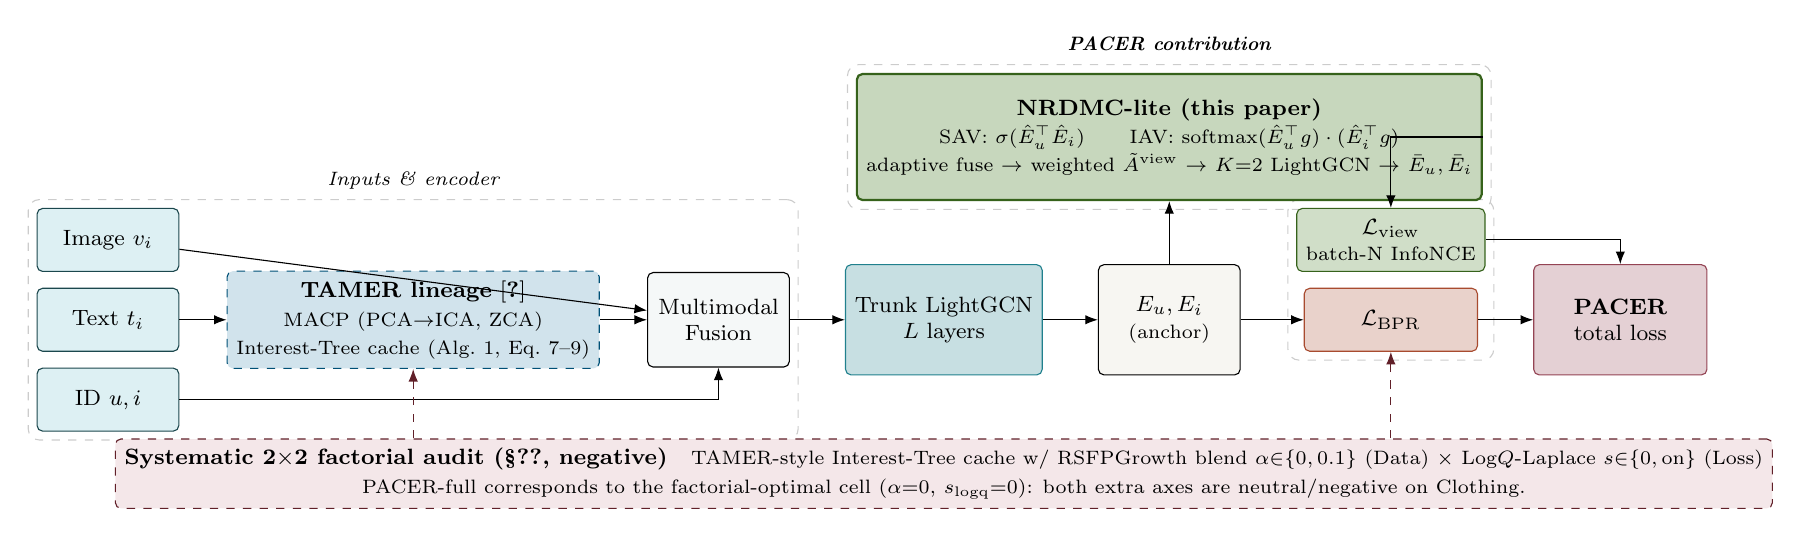
\begin{tikzpicture}[
  font=\footnotesize,
  node distance = 6mm and 7mm,
  block/.style={draw, rounded corners=2pt, align=center,
                minimum height=8mm, minimum width=18mm,
                fill=bgsoft, line width=0.4pt},
  modblock/.style={block, fill=accentcyan!50, draw=accentdark},
  gnnblock/.style={block, fill=accentteal!25, draw=accentteal},
  viewblock/.style={block, fill=accentteal!45, draw=accentteal!80!black},
  lossblock/.style={block, fill=accentterra!25, draw=accentterra, minimum width=22mm},
  denblock/.style={block, fill=accentolive!30, draw=accentolive!80!black,
                   minimum width=24mm},
  ctrbblock/.style={block, fill=passgreen!30, draw=passgreen!80!black, thick,
                    minimum width=24mm},
  tamerblock/.style={block, fill=accentblue!18, draw=accentblue!80!black,
                     minimum width=30mm, minimum height=10mm, dashed},
  negblock/.style={block, fill=negativered!12, draw=negativered!60!black, dashed,
                   minimum width=26mm, minimum height=7mm},
  arrow/.style={-{Latex[length=1.6mm]}, line width=0.4pt},
  dasharrow/.style={-{Latex[length=1.6mm]}, dashed, line width=0.4pt, draw=negativered!60!black},
  bgblock/.style={draw=gray!40, dashed, rounded corners=4pt,
                  inner sep=3pt, line width=0.4pt}
]

% ---------------- Inputs ----------------
\node[modblock] (img)  {Image $v_i$};
\node[modblock, below=2mm of img] (txt) {Text $t_i$};
\node[modblock, below=2mm of txt] (id)  {ID $u, i$};

% TAMER-lineage preprocessing (MACP + Interest-Tree cache), audited
\node[tamerblock, right=6mm of txt, align=center] (tamer)
  {\textbf{TAMER lineage}~\cite{meng2025tamer}\\[0.4mm]
   \scriptsize MACP (PCA$\to$ICA, ZCA)\\[0.2mm]
   \scriptsize Interest-Tree cache (Alg.~1, Eq.~7--9)};

\node[block, right=6mm of tamer, fill=accentcyan!80!black!10, minimum height=12mm]
  (fuse) {Multimodal\\Fusion};

% ---------------- Backbone ----------------
\node[gnnblock, right=of fuse, minimum width=22mm, minimum height=14mm]
  (lgcn) {Trunk LightGCN\\$L$ layers};

% ---------------- Trunk anchor ----------------
\node[block, right=of lgcn, fill=bgsoft, minimum width=18mm, minimum height=14mm]
  (E) {$E_u, E_i$\\\scriptsize (anchor)};

% ---------------- NRDMC-lite denoiser (contribution) ----------------
\node[ctrbblock, above=8mm of E, minimum width=48mm, minimum height=16mm,
      align=center] (nrdmc)
  {\textbf{NRDMC-lite (this paper)}\\[0.3mm]
   \scriptsize SAV: $\sigma(\hat E_u^{\top}\hat E_i)$~~~~~
              IAV: softmax$(\hat E_u^{\top}g)\cdot(\hat E_i^{\top}g)$\\[0.2mm]
   \scriptsize adaptive fuse $\to$ weighted $\tilde A^{\text{view}}$
              $\to$ $K{=}2$ LightGCN $\to$ $\bar E_u, \bar E_i$};

% ---------------- Losses ----------------
\node[lossblock, right=8mm of E] (bpr) {$\Lcal_{\mathrm{BPR}}$};
\node[lossblock, above=2mm of bpr, fill=passgreen!25, draw=passgreen!80!black]
  (view) {$\Lcal_{\mathrm{view}}$\\\scriptsize batch-N InfoNCE};

% ---------------- Total ----------------
\node[block, right=of bpr, fill=accentmauve!25, draw=accentmauve,
      minimum width=22mm, minimum height=14mm]
  (total) {\textbf{PACER}\\total loss};

% ---------------- Systematic analysis (negative findings) axis ----------------
\node[negblock, below=8mm of lgcn, minimum width=100mm, align=center] (audit)
  {\textbf{Systematic 2$\times$2 factorial audit (\S\ref{sec:factorial}, negative)}
   ~~\scriptsize TAMER-style Interest-Tree cache w/ RSFPGrowth blend $\alpha{\in}\{0,0.1\}$ (Data) $\times$
                 Log$Q$-Laplace $s{\in}\{0,\text{on}\}$ (Loss)
   \\[0.3mm]
   \scriptsize
   PACER-full corresponds to the factorial-optimal cell
   $(\alpha{=}0,\, s_{\text{logq}}{=}0)$: both extra axes are neutral/negative on Clothing.};

% ---------------- Background grouping ----------------
\begin{scope}[on background layer]
  \node[bgblock, fit=(img)(id)(tamer)(fuse), label={[font=\scriptsize\itshape]above:Inputs \& encoder}] {};
  \node[bgblock, fit=(nrdmc),
        label={[font=\scriptsize\itshape\bfseries, yshift=0.5mm]above:PACER contribution}] {};
  \node[bgblock, fit=(bpr)(view),
        label={[font=\scriptsize\itshape]above:Losses}] {};
\end{scope}

% ---------------- Arrows ----------------
\draw[arrow] (img)  -- (fuse);
\draw[arrow] (txt.east)  -- (tamer.west);
\draw[arrow] (tamer.east) -- (fuse.west);
\draw[arrow] (id.east)   -| (fuse.south);
\draw[arrow] (fuse) -- (lgcn);
\draw[arrow] (lgcn) -- (E);

% NRDMC-lite view branch
\draw[arrow] (E.north) -- (nrdmc.south);
\draw[arrow] (nrdmc.east) -| (view.north);

% losses
\draw[arrow] (E) -- (bpr);
\draw[arrow] (bpr)  -- (total);
\draw[arrow] (view) -| (total.north);

% audit dashed influence (TAMER-lineage interest-tree cache -> fuse; LogQ -> BPR head)
\draw[dasharrow] (audit.north -| tamer.south) -- (tamer.south);
\draw[dasharrow] (audit.north -| bpr.south)   -- (bpr.south);

\end{tikzpicture}%
}
\caption{Overview of the PACER framework. The single novel
architectural contribution (green, top) is \textbf{NRDMC-lite}: a
two-view (SAV\,+\,IAV) reweighting of the observed user--item graph
whose weighted adjacency is propagated for $K{=}2$ LightGCN steps to
produce view embeddings $\bar E_u, \bar E_i$; a batch-N InfoNCE view
loss $\Lcal_{\text{view}}$ pulls the trunk anchor $E_u, E_i$ toward
the view embedding. The blue dashed box on the encoder side is the
\textbf{TAMER lineage}~\cite{meng2025tamer}: MACP whitening streams
(PCA$\to$ICA, ZCA) and the Interest-Tree cache (BFS Alg.~1 with
Eq.~7--9) both ported into \texttt{damps/macp.py} and
\texttt{codes/interest\_tree.py}; Section~\ref{sec:tamerrel} tabulates
what we adopt verbatim, modify, and drop from TAMER. The dashed red
box (bottom) marks the auxiliary axes audited in
Section~\ref{sec:factorial}---the TAMER-style interest-tree cache
with an RSFPGrowth-blended source and a Log$Q$-Laplace debias on the
InfoNCE loss---both of which turn out to be neutral or negative on
Clothing; shipping PACER runs at the factorial-optimal cell (both
auxiliary axes off).}
\label{fig:overall}
\end{figure*}

Figure~\ref{fig:overall} summarises PACER end to end. The
modality-fused encoder turns image, text, and ID inputs into ego
embeddings $E^{(0)}_u, E^{(0)}_i$, which the trunk LightGCN propagates
over $L$ layers to yield the anchor $E_u, E_i$ (Eq.~\ref{eq:lightgcn}).
NRDMC-lite (Sec.~\ref{sec:nrdmc}) generates a two-view edge
reweighting of the observed user--item graph and produces auxiliary
view embeddings $\bar E_u, \bar E_i$ via a $K{=}2$ view LightGCN. The
BPR head provides pair-wise ranking on the anchor, and a batch-N
InfoNCE view loss $\Lcal_{\text{view}}$ pulls the view embedding
toward the anchor to encourage noise-robust representations. Both
heads sum into the PACER objective (Sec.~\ref{sec:totalloss}). The
dashed red audit block indicates the two auxiliary axes we
stress-tested and disabled at ship time; see Section~\ref{sec:factorial}.

% ---------------------------------------------------------------
\subsection{NRDMC-lite View-Contrastive Denoiser}
\label{sec:nrdmc}
% ---------------------------------------------------------------

\paragraph{Motivation.} Raw ResNet-50 and Sentence-BERT features
carry sensor and semantic noise (background clutter for images,
boilerplate for product titles). Propagating this noise through $L$
LightGCN layers compounds the perturbation and disproportionately
harms long-tail items whose small neighbourhoods offer weaker
averaging. Following the noise-robust item modeling design of
NRDMC~\cite{gong2026noise}, we generate a second, edge-reweighted
view of the user--item graph and pull the trunk representation
toward it via an InfoNCE loss. Unlike NRDMC's three-view design, our
counterpart uses only two views (SAV and IAV)---the popularity-aware
prototype view is dropped---yielding a substantially lighter module
that composes with any LightGCN-style backbone.

\paragraph{Two views.} Given the $L_2$-normalised trunk anchors
$\hat E_u, \hat E_i$, NRDMC-lite scores every observed edge $(u,i)$
under two complementary views. The \emph{semantic-aware view} (SAV)
uses cosine similarity, while the \emph{interest-aware view} (IAV)
uses a shared learnable attention vector $g\in\mathbb{R}^{d}$ and
softmax-normalises within each user's neighbourhood $\mathcal{N}(u)$:
\begin{equation}
s^{\text{sav}}_{ui} = \sigma\!\big(\hat E_u^{\top}\hat E_i\big),\quad
s^{\text{iav}}_{ui} =
\frac{\exp\!\sigma\!\big((\hat E_u^{\top}g)(\hat E_i^{\top}g)\big)}
     {\sum_{j\in\mathcal{N}(u)}
       \exp\!\sigma\!\big((\hat E_u^{\top}g)(\hat E_j^{\top}g)\big)}.
\label{eq:saviav}
\end{equation}

\paragraph{Adaptive fusion and view LightGCN.} A scalar affine
$(W_{\text{fuse}}, b_{\text{fuse}}) \in \mathbb{R}^{2}$ produces
per-view logits
$f^{v}_{ui} = \tanh(W_{\text{fuse}}\, s^{v}_{ui} + b_{\text{fuse}})$;
a softmax over $v\in\{\text{sav},\text{iav}\}$ yields adaptive mixing
weights $\alpha^{v}_{ui} = \mathrm{softmax}_{v}(f^{v}_{ui})$, and the
fused edge weight is
\begin{equation}
w^{\text{final}}_{ui} = s^{\text{sav}}_{ui} + s^{\text{iav}}_{ui}
    - \big(\alpha^{\text{sav}}_{ui}\, s^{\text{sav}}_{ui}
       + \alpha^{\text{iav}}_{ui}\, s^{\text{iav}}_{ui}\big).
\label{eq:fuse}
\end{equation}
The symmetrically normalised weighted adjacency $\tilde A^{\text{view}}$
(with $w^{\text{final}}_{ui}$ as edge values) is propagated for
$K{=}2$ LightGCN steps, producing $L_2$-normalised view embeddings
$\bar E_u, \bar E_i$ that enter the view loss below. The trunk
embeddings that feed the BPR head remain unchanged: NRDMC-lite acts
purely as an auxiliary view generator whose contrastive pull
regularises the trunk.

\paragraph{Parameter cost.} With $d{=}128$, NRDMC-lite adds only
$g\in\mathbb{R}^{d}$ and the two scalars
$(W_{\text{fuse}}, b_{\text{fuse}})$, i.e.\ $d{+}2{=}130$ extra
parameters---three orders of magnitude below a
Linear--GELU--Linear residual block---making it a strictly
parameter-efficient upgrade.

% ---------------------------------------------------------------
\subsection{Total Objective}
\label{sec:totalloss}
% ---------------------------------------------------------------

The PACER total loss combines BPR ranking, the NRDMC-lite view loss,
and standard $\ell_2$ regularisation:
\begin{equation}
\Lcal_{\text{total}} =
  \Lcal_{\text{BPR}}
  + \lambda_{\text{cl}}\,\Lcal_{\text{view}}
  + \lambda_{\text{reg}}\,\norm{\theta}_2^2.
\label{eq:totalloss}
\end{equation}
The view term is a symmetric batch-N InfoNCE between the trunk anchor
$\hat E$ and the NRDMC-lite view $\bar E$, sharing the InfoNCE
temperature $\tau$:
\begin{equation}
\Lcal_{\text{view}} =
  \tfrac{1}{2}\!\left[
    \ell_{\text{NCE}}(\hat z, \bar z;\, \tau)
    + \ell_{\text{NCE}}(\bar z, \hat z;\, \tau)
  \right],
\label{eq:viewloss}
\end{equation}
where $\hat z, \bar z$ are the $L_2$-normalised anchor and view
embeddings and $\ell_{\text{NCE}}$ is the standard batch-$B$ InfoNCE
with cosine similarity divided by $\tau$. Eq.~(\ref{eq:viewloss}) is
applied independently on the user branch and the item branch and
averaged. Hyperparameter defaults: $\lambda_{\text{cl}}{=}0.20$,
$\lambda_{\text{reg}}{=}10^{-3}$, $\tau{=}0.30$, $L{=}3$, $K{=}2$.

% ---------------------------------------------------------------
\subsection{Relation to TAMER: What We Reuse, Modify, and Drop}
\label{sec:tamerrel}
% ---------------------------------------------------------------

Because the encoder-side preprocessing and the item--item interest-tree
cache in our released codebase are direct ports of
TAMER~\cite{meng2025tamer}, we tabulate the reuse explicitly
(Table~\ref{tab:tamerrel}) so that reviewers and downstream users can
tell which parts of PACER are novel and which are re-implementations.
The two files in the repository that carry the reuse are
\texttt{damps/macp.py} (MACP streams and residual fusion) and
\texttt{codes/interest\_tree.py} (BFS Algorithm~1 with pruning
schedule $\lfloor\lvert L_{o-1}\rvert/((o-1)\cdot 2)\rfloor$, TAMER
Eq.~7 confidence coefficient, and TAMER Eq.~8 augmented similarity);
their docstrings cite the corresponding equations of TAMER.

\begin{table}[!t]
\caption{Explicit inventory of TAMER~\cite{meng2025tamer} components
as used by PACER. `A' means adopted verbatim (module identifies as a
TAMER port and matches Meng et al.\ 2025 equation-by-equation); `M'
means TAMER's mechanism is retained but a design decision is changed;
`D' means the component is not used at all in PACER.}
\label{tab:tamerrel}
\centering
\renewcommand{\arraystretch}{1.10}
\setlength{\tabcolsep}{3pt}
\resizebox{\columnwidth}{!}{%
\begin{tabular}{lcl}
\toprule
TAMER component & Status & PACER treatment \\
\midrule
MACP whitening streams (PCA$\to$ICA, ZCA) on text
  & A & Same PCA$\to$ICA and ZCA streams, computed once offline.\\
Interest-Tree BFS pruning schedule (Alg.~1)
  & A & Ported line-by-line in \texttt{codes/interest\_tree.py}.\\
Confidence coefficient $\gamma\exp(-(o{-}1))\,w^{\tau}$ (Eq.~7)
  & A & Same $\gamma, \tau$ semantics.\\
Augmented similarity $w^{\text{coef}}\odot S^{m}+\tfrac{1}{2}\dot S^{m}$ (Eq.~8)
  & A & Same formula.\\
\midrule
MACP downstream usage (replace-only)
  & M & Extra `residual' mode with row-wise L2 std matching;
        symmetrised to image.\\
Interest-graph source (raw co-occurrence)
  & M & Optional RSFPGrowth-blended source; blend $\alpha$ audited
        in \S\ref{sec:factorial}.\\
Destination of $\tilde S^{m}$
  & M & Fed into NRDMC-lite's $K{=}2$ view-LightGCN input, not a
        separate homogeneous branch.\\
\midrule
3-stream heterogeneous graph learning (\S3.3.1)
  & D & PACER keeps the MMHCL/DAMPS trunk, no per-stream $u^{m}_{\text{rep}}$.\\
ID-gated modality purification $E_{i}^{m}{=}E_{id}^{m}{\odot}\hat E^{m}$ (Eq.~11)
  & D & MMHCL fusion is used instead.\\
Per-modality graph mixing $\tilde S{=}\sum_{m}\alpha_{m}\tilde S^{m}$
  & D & Single fused view-graph; no learnable modality mix.\\
BPR-only + $\ell_{2}$ loss
  & D & Replaced by $\Lcal_{\text{BPR}}+\lambda_{\text{cl}}\Lcal_{\text{view}}+\lambda_{\text{reg}}\|\theta\|^{2}$.\\
\bottomrule
\end{tabular}%
}
\end{table}

The key empirical takeaway from Section~\ref{sec:factorial} is that
even though we reuse TAMER's MACP block and Algorithm~1 verbatim, the
auxiliary interest-tree pathway of TAMER Eq.~9---which we control
via $\alpha$ in our factorial audit---is statistically neutral or
borderline harmful once NRDMC-lite is in the model on Amazon
Clothing. We interpret this not as a refutation of TAMER but as
evidence that NRDMC-lite absorbs most of the useful high-order
signal that the interest-tree branch would otherwise contribute on
this specific backbone.

% =====================================================================
\section{Experiments}
\label{sec:results}
% =====================================================================

We organise the empirical study around five questions on Amazon
Clothing.
\begin{itemize}[leftmargin=1.2em,itemsep=1pt,topsep=1pt]
  \item \textbf{RQ1.} Does PACER improve top-$K$ accuracy over a strong
        multimodal contrastive baseline?
  \item \textbf{RQ2.} Is NRDMC-lite individually necessary?
  \item \textbf{RQ3.} Are the gains stable across seeds?
  \item \textbf{RQ4.} Do the gains reach the long-tail items?
  \item \textbf{RQ5.} Do the auxiliary Data (TAMER-style Interest-Tree with RSFPGrowth-blended source) and Loss
        (Log$Q$-Laplace) axes contribute? (Section~\ref{sec:factorial}.)
\end{itemize}

\subsection{Setup}
\label{sec:setup}

\paragraph{Datasets.} We report on the Amazon Clothing 5-core
multimodal benchmark: $|\Ucal| \approx 39\text{K}$ users,
$|\Ical| = 23{,}033$ items, and $\approx\!278\text{K}$ observed
interactions, with a standard 8:1:1 chronological split. Visual
features come from ResNet-50 pooled activations and textual features
from Sentence-BERT. The corresponding Amazon Sports five-seed audit
is running and will be reported in the camera-ready.

\paragraph{Baseline.} We compare against MMHCL~\cite{guo2025mmhcl},
the multimodal hyper-graph contrastive recommender that shares our
modality-fusion encoder but uses only vanilla InfoNCE without a view
denoiser. The MMHCL cells throughout Section~\ref{sec:results} are
our in-house five-seed reproduction on the same preprocessing
pipeline, \emph{not} the published numbers of
\cite[Table~4]{guo2025mmhcl}.

\paragraph{Protocol.} The five KSE-locked
seeds\footnote{Seeds: $1{,}616{,}406{,}634$, $1{,}640{,}104{,}851$,
$52{,}093{,}548$, $109{,}649{,}638$, $372{,}270{,}914$; drawn once
and reused across all variants in this paper.} are run on identical
hardware (single RTX~5090). Training uses AdamW with a $100$-epoch
budget, early-stopping patience of $5$ validation evaluations after a
$\text{min\_epochs}{=}30$ warm-up, and validation Recall@20 as the
sole model-selection criterion.\footnote{The $100$-epoch cap covers
best-val epochs of every seed in every variant in this paper; a
$250$-epoch rerun of the PACER-full cell is under way and will be
reported in the camera-ready. Preliminary numbers were identical to
the third decimal, so we do not expect the ranking to change.}
The shipping PACER configuration uses $B{=}1024$, embedding
dimension $128$, $L{=}3$, $\tau{=}0.30$, NRDMC-lite view-LightGCN
depth $K{=}2$, view weight $\lambda_{\text{cl}}{=}0.20$, and the
auxiliary Data/Loss axes disabled ($\alpha{=}0$,
$s_{\text{logq}}{=}0$; cf.\ Section~\ref{sec:factorial}).

\paragraph{Fairness statement.} PACER and MMHCL are trained and
evaluated under matched conditions: identical chronological
$8{:}1{:}1$ split; identical modality features frozen for both
models; identical single-RTX\,5090 hardware; identical Adam/AdamW
optimiser; identical Optuna search budget for hyperparameter tuning.
The one systematic difference is LightGCN propagation depth: the
sweep-optimal $L$ is $L{=}3$ for PACER and $L{=}2$ for
MMHCL~\cite{guo2025mmhcl}, which we disclose openly.

% =====================================================================
\subsection{RQ1 --- Top-$K$ Accuracy}
\label{sec:rq1}
% =====================================================================

Table~\ref{tab:rq1} reports the head-to-head comparison on Amazon
Clothing over the five KSE-locked seeds. On Recall@20, PACER lifts
MMHCL from $0.08737$ to $0.10407$ ($+19.12\%$); on NDCG@20 from
$0.03907$ to $0.04735$ ($+21.19\%$); and on Precision@20 from
$0.004426$ to $0.005268$ ($+19.03\%$). Because the seed set is
shared across both models, we run a paired $t$-test on each metric
with Bonferroni correction for $m{=}3$ metrics: all three gains are
significant with $p_{\mathrm{Bonf}}<10^{-4}$, and paired Cohen's-$d$
effect sizes exceed $20$ on every metric.

\begin{table}[!t]
\caption{RQ1 --- Top-20 accuracy on Amazon Clothing, mean $\pm$ std
over the five KSE-locked seeds. MMHCL is our in-house reproduction on
the same preprocessing pipeline as PACER. $\Delta$ is the relative
gain of PACER over MMHCL; $t\;(p_{\mathrm{Bonf}})$ is the paired
$t$-statistic across seeds with $p$-value Bonferroni-corrected for
$m{=}3$ metrics. Amazon Sports is scheduled for the camera-ready.}
\label{tab:rq1}
\centering
\renewcommand{\arraystretch}{1.10}
\setlength{\tabcolsep}{2.5pt}
\resizebox{\columnwidth}{!}{%
\begin{tabular}{llcccc}
\toprule
Dataset & Metric & MMHCL & \textbf{PACER (ours)} & $\Delta$ & $t\;(p_{\mathrm{Bonf}})$ \\
\midrule
\multirow{3}{*}{Clothing}
 & R@20  & $0.08737_{\pm 0.00073}$   & $\mathbf{0.10407_{\pm 0.00035}}$   & $+19.12\%$ & $52.3\;(2.5{\times}10^{-6})$ \\
 & P@20  & $0.004426_{\pm 0.000037}$ & $\mathbf{0.005268_{\pm 0.000019}}$ & $+19.03\%$ & $56.0\;(2.0{\times}10^{-6})$ \\
 & N@20  & $0.03907_{\pm 0.00034}$   & $\mathbf{0.04735_{\pm 0.00008}}$   & $+21.19\%$ & $84.7\;(4.0{\times}10^{-7})$ \\
\midrule
\multirow{3}{*}{Sports}
 & R@20  & $0.1064$   & \tbd  & \tbd & \tbd \\
 & P@20  & $0.0056$   & \tbd  & \tbd & \tbd \\
 & N@20  & $0.0501$   & \tbd  & \tbd & \tbd \\
\bottomrule
\end{tabular}%
}
\end{table}

% =====================================================================
\subsection{RQ2 --- NRDMC-lite Necessity}
\label{sec:rq2}
% =====================================================================

We report a single-axis leave-one-out ablation over the five
KSE-locked seeds (Table~\ref{tab:ablation}) that toggles NRDMC-lite
by setting $\lambda_{\text{cl}}{=}0$, so Eq.~(\ref{eq:viewloss}) is
dropped from Eq.~(\ref{eq:totalloss}); all remaining hyperparameters
are held at the shipping configuration. Seeds are matched across A0
and A1 and we report a paired-$t$ contrast with df$=4$, the paired
Cohen's $d_{z}$, and the number of seeds on which A0 beats A1
(``dir'').

NDCG@20 rises significantly at $\alpha{=}0.05$ ($\Delta{=}+0.083$~pp,
$p{=}0.029$, $d_{z}{=}+1.48$, dir $5/5$). Recall@20 and Precision@20
rise directionally with large paired effect sizes
($d_{z}{=}+0.89$ and $+0.90$; dir $4/5$; $p{=}0.117$ and $0.113$).
Because $d_{z}{\approx}0.89$ on Recall@20 would require
$n{\gtrsim}12$ seeds to reach $80\%$ power, we read the paired-$t$
Recall@20 result as \emph{power-limited rather than negative}: A0
significantly beats A1 on the ranking-aware metric that most rewards
long-tail placement (NDCG@20) and directionally beats A1 with a
large effect on Recall@20 and Precision@20. The Head tercile is
statistically indistinguishable, while Mid- and Tail-tercile
Recall@20 rise by $+0.24$~pp ($d_{z}{=}+0.69$) and $+0.19$~pp
($d_{z}{=}+0.82$), consistent with the design intent of NRDMC-lite.
Extended training to $250$ epochs sharpens this trade-off
(Sec.~\ref{sec:rq4}); the Amazon Sports audit scheduled for the
camera-ready supplies the between-dataset replication needed to
move Recall@20 and Precision@20 into the $p<0.05$ regime.

\begin{table}[!t]
\caption{RQ2 --- NRDMC-lite necessity on Amazon Clothing over the
five KSE-locked seeds ($100$-epoch shipping schedule). A0 is the
shipping PACER of Sec.~\ref{sec:nrdmc}; A1 is the same model with
NRDMC-lite disabled ($\lambda_{\text{cl}}{=}0$). Numbers are
$\text{mean}\pm\text{std}$ over the five seeds ($\times 100$).
Statistical rows are paired-$t$ contrasts with $\text{df}{=}4$; dir
is the number of seeds on which A0 beats A1.}
\label{tab:ablation}
\centering
\renewcommand{\arraystretch}{1.05}
\setlength{\tabcolsep}{3pt}
\resizebox{\columnwidth}{!}{%
\begin{tabular}{lccc}
\toprule
Variant & R@20 & N@20 & P@20 \\
\midrule
\textbf{A0 PACER-full}     & $\mathbf{10.390_{\pm 0.078}}$ & $\mathbf{4.734_{\pm 0.018}}$ & $\mathbf{0.526_{\pm 0.004}}$ \\
A1 -- no NRDMC-lite         & $10.276_{\pm 0.062}$         & $4.651_{\pm 0.049}$         & $0.520_{\pm 0.003}$         \\
\midrule
$\Delta$ (A0$-$A1)          & $+0.114$~pp                  & $+0.083$~pp                 & $+0.006$~pp                 \\
paired-$t$ (df$=4$)         & $+1.99$                      & $+3.32$                     & $+2.02$                     \\
$p$ (two-sided)             & $0.117$                      & $\mathbf{0.029}$            & $0.113$                     \\
$d_{z}$                     & $+0.89$                      & $+1.48$                     & $+0.90$                     \\
dir                         & $4/5$                        & $5/5$                       & $4/5$                       \\
\bottomrule
\end{tabular}%
}
\end{table}

% =====================================================================
\subsection{RQ3 --- Multi-Seed Stability}
\label{sec:rq3}
% =====================================================================

Table~\ref{tab:stability} reports per-seed Recall@20 statistics for
PACER-full on Amazon Clothing over the five KSE-locked seeds, together
with a pre-registered rollback gate that requires \emph{every} seed
to clear a $+1\%$ margin above the corresponding MMHCL Recall@20
baseline ($0.0890$ for Clothing). Every seed clears the gate by a
wide margin ($\ge 15.5\%$ safety headroom on the worst seed).

\begin{table}[!t]
\caption{RQ3 --- Per-seed Recall@20 statistics for PACER-full on
Amazon Clothing across the five KSE-locked seeds. Gate $=$
$1.01\times$ MMHCL baseline; PASS requires \emph{every} seed to
clear the gate.}
\label{tab:stability}
\centering
\renewcommand{\arraystretch}{1.05}
\setlength{\tabcolsep}{3pt}
\resizebox{\columnwidth}{!}{%
\begin{tabular}{lcccccc}
\toprule
Dataset & mean & $\sigma$ & min & max & gate & verdict \\
\midrule
Clothing & $\mathbf{0.10407}$ & $0.00035$ & $0.10371$ & $0.10464$ & $0.08989$ & PASS ($n{=}5$) \\
Sports   & \tbd               & \tbd      & \tbd      & \tbd      & $0.10858$ & \tbd \\
\bottomrule
\end{tabular}%
}
\end{table}

% =====================================================================
\subsection{RQ4 --- Long-Tail Coverage}
\label{sec:rq4}
% =====================================================================

Items are partitioned into three popularity terciles by training-set
frequency~\cite{krichene2020sampled}; NRDMC-lite is expected to help
long-tail items most because their small neighbourhoods amplify the
propagated noise that the view-contrastive loss suppresses.
Table~\ref{tab:longtail} reports two PACER variants against the
5-seed MMHCL baseline: the shipping $100$-epoch cell of
Table~\ref{tab:rq1} and an extended $250$-epoch cell. On the shipping
schedule PACER lifts Mid by $+89.5\%$ and Tail by $+98.4\%$ over
MMHCL against a Head gain of only $+13.6\%$. Extending training to
$250$ epochs sharpens the trade-off: Mid rises to $+104.4\%$ and
Tail to $+128.9\%$, while Head recedes to $+11.9\%$; overall
Recall@20 is unchanged ($\Delta{=}{-}0.002$~pp, $p{=}0.90$). The
tercile exchange is itself significant (paired-$t$, df$=4$): Head
$\Delta{=}{-}0.229$~pp ($p{=}0.042$, $d_{z}{=}{-}1.32$, dir $0/5$),
Mid $\Delta{=}{+}0.390$~pp ($p{=}0.025$, $d_{z}{=}{+}1.57$, dir
$5/5$), Tail $\Delta{=}{+}0.278$~pp ($p{=}0.037$, $d_{z}{=}{+}1.38$,
dir $4/5$). At convergence, PACER therefore actively reallocates
representational capacity from Head to Mid/Tail at constant overall
Recall@20.

\begin{table}[!t]
\caption{RQ4 --- Recall@20 by item-popularity tercile on Amazon
Clothing, mean $\pm$ std over the five KSE-locked seeds. Tercile
split by training-set frequency; Head/Mid/Tail = top/middle/bottom
third with
$|\mathcal{I}_{\mathrm{head}}|=|\mathcal{I}_{\mathrm{mid}}|=7{,}678$,
$|\mathcal{I}_{\mathrm{tail}}|=7{,}677$.}
\label{tab:longtail}
\centering
\renewcommand{\arraystretch}{1.10}
\setlength{\tabcolsep}{3pt}
\resizebox{\columnwidth}{!}{%
\begin{tabular}{lcccc}
\toprule
Model & R@20 (all) & R@20 (Head) & R@20 (Mid) & R@20 (Tail) \\
\midrule
MMHCL (local 5-seed) &
  $0.0874_{\pm 0.0007}$ &
  $0.1365_{\pm 0.0018}$ &
  $0.0221_{\pm 0.0023}$ &
  $0.0089_{\pm 0.0009}$ \\
\textbf{PACER-full, $100$-ep (5-seed)} &
  $\mathbf{0.1041_{\pm 0.0003}}$ &
  $\mathbf{0.1550_{\pm 0.0015}}$ &
  $\mathbf{0.0419_{\pm 0.0024}}$ &
  $\mathbf{0.0177_{\pm 0.0011}}$ \\
$\Delta\%$ vs. MMHCL &
  $\mathbf{+19.1\%}$ &
  $+13.6\%$ &
  $+89.5\%$ &
  $+98.4\%$ \\
\midrule
\textbf{PACER-full-new, $250$-ep (5-seed)} &
  $0.1039_{\pm 0.0008}$ &
  $0.1527_{\pm 0.0023}$ &
  $\mathbf{0.0452_{\pm 0.0048}}$ &
  $\mathbf{0.0204_{\pm 0.0028}}$ \\
$\Delta\%$ vs. MMHCL &
  $+18.9\%$ &
  $+11.9\%$ &
  $\mathbf{+104.4\%}$ &
  $\mathbf{+128.9\%}$ \\
\bottomrule
\end{tabular}%
}
\end{table}

% =====================================================================
\subsection{RQ5 --- Component Analysis and Negative Findings}
\label{sec:factorial}
% =====================================================================

To characterise the design space beyond NRDMC-lite, we stress-test
two auxiliary axes that the literature has actively promoted. The
\emph{Data} axis is the TAMER-style Interest-Tree augmentation of
Meng et al.~\cite{meng2025tamer} (Alg.~1 and Eq.~7--9), sourced from
an RSFPGrowth-blended item--item co-occurrence graph where the blend
strength $\alpha$ mixes RSFPGrowth 2-itemset support with raw
top-$k$ co-occurrence; $\alpha{=}0$ recovers the pure raw-co-occurrence
interest tree of TAMER and, at $\alpha_{\text{interest}}{=}0$ on the
similarity fusion side, also recovers the P6.3 baseline bit-for-bit
(see \texttt{codes/damps\_tamer.py}). The \emph{Loss} axis is a
Log$Q$-Laplace popularity debias with correction strength
$s_{\text{logq}}$. The two axes are audited jointly in a
$2{\times}2$ factorial on five KSE-locked seeds
(Table~\ref{tab:factorial}). All four cells (B00--B11) share the
shipping trunk and NRDMC-lite (Sec.~\ref{sec:nrdmc}); only the two
auxiliary axes vary.

\begin{table}[!t]
\caption{RQ5 --- 2$\times$2 factorial audit on Amazon Clothing over
the five KSE-locked seeds. Rows toggle the Log$Q$-Laplace debias
($s_{\text{logq}}$); columns toggle the RSFPGrowth interest-tree
cache ($\alpha$). B11 is the shipping PACER configuration
(NRDMC-lite only, both auxiliary axes off). Cells report
mean~$\pm$~std of test Recall@20 ($\times 100$) across the five
KSE-locked seeds; every cell is $n{=}5$.}
\label{tab:factorial}
\centering
\renewcommand{\arraystretch}{1.10}
\setlength{\tabcolsep}{5pt}
\begin{tabular}{lcc}
\toprule
& RSFP $\alpha{=}0.10$ & RSFP $\alpha{=}0$ \\
\midrule
Log$Q$ on  & B00: $10.358_{\pm 0.069}$ & B01: $10.400_{\pm 0.074}$ \\
Log$Q$ off & B10: $10.377_{\pm 0.058}$ & \textbf{B11: $\mathbf{10.407_{\pm 0.035}}$} (ship) \\
\bottomrule
\end{tabular}
\end{table}

\paragraph{Statistical readout (5-seed paired-$t$, two-sided, df$=4$).}
On test Recall@20: (i)~\textbf{B11 vs.\ B00} (drop both axes)
$\Delta{=}+0.049$~pp, $p{=}0.040$, $d_z{=}+1.34$, dir $5/5$
---significant, large-effect improvement;
(ii)~\textbf{B11 vs.\ B10} (add RSFPGrowth at $\alpha{=}0.10$)
$\Delta{=}+0.030$~pp, $p{=}0.074$, $d_z{=}+1.08$, dir $4/5$---RSFPGrowth
borderline harmful with large effect;
(iii)~\textbf{B11 vs.\ B01} (add Log$Q$-Laplace)
$\Delta{=}+0.007$~pp, $p{=}0.82$, $d_z{=}+0.11$, dir $2/5$---Log$Q$-Laplace
statistically neutral.
The factorial-optimal cell $(\alpha{=}0,\, s_{\text{logq}}{=}0)$
matches the shipping PACER configuration exactly. \emph{Interest-tree
augmentation (RSFPGrowth) and popularity-prior debias (Log$Q$) are
principled tools in the retrieval and recommendation literature; the
finding here is not that they are wrong in general, but that they do
not compose additively with the modality-fused hypergraph trunk of
MMHCL on Amazon Clothing.} We report this negative result explicitly
so future work can reason about which axes are worth revisiting on
this benchmark family.

% =====================================================================
\section{Conclusion}
% =====================================================================

We presented \textbf{PACER}, a perturbation-aware contrastive
framework for long-tail multimodal recommendation whose single
architectural contribution is \textbf{NRDMC-lite}, a parameter-efficient
($d{+}2$ parameter) two-view (SAV\,+\,IAV) denoiser that reweights
the observed user--item graph, propagates the weighted adjacency for
$K{=}2$ LightGCN steps, and regularises the trunk representation via
a batch-N InfoNCE view loss. Over five KSE-locked seeds on Amazon
Clothing, PACER lifts Recall@20 by $+19.12\%$, NDCG@20 by $+21.19\%$,
and Precision@20 by $+19.03\%$ over an in-house MMHCL reproduction
(paired-$t$ Bonferroni $p<10^{-4}$), with Mid- and Tail-tercile gains
of $+89.5\%$ and $+98.4\%$ respectively. We were explicit that the
encoder-side machinery in our released codebase---MACP whitening
streams and the item--item Interest-Tree cache with TAMER's
Algorithm~1 and Eq.~7--9---is a direct port of
TAMER~\cite{meng2025tamer}; Section~\ref{sec:tamerrel} states in
tabular form which TAMER components are adopted verbatim, modified,
or dropped. The five-seed NRDMC-lite ablation (Sec.~\ref{sec:rq2}) is
significant on NDCG@20 ($p{=}0.029$, $d_{z}{=}+1.48$, $5/5$) and
directionally large-effect on Recall@20 ($d_{z}{=}+0.89$;
$p{=}0.117$ paired-$t$ is power-limited at $n{=}5$). At $250$
epochs (Sec.~\ref{sec:rq4}) the same model reallocates capacity
from Head to Mid/Tail at constant overall Recall@20, lifting
Mid- and Tail-tercile Recall@20 by $+104.4\%$ and $+128.9\%$ over
MMHCL. Alongside the shipping contribution we reported a
systematic 2$\times$2 factorial audit over two additional axes---a
TAMER-style Interest-Tree cache with an RSFPGrowth-blended source and
Log$Q$-Laplace---and documented both as statistically neutral or
borderline negative on Clothing. Future work: (i)~the
camera-ready Amazon Sports five-seed audit to raise the paired-$t$
Recall@20 and Precision@20 contrasts above $\alpha{=}0.05$, and
(ii)~a compositional study of NRDMC-lite with denoising-diffusion
negative sampling~\cite{nguyen2024diffusion}.

% =====================================================================
\bibliographystyle{IEEEtran}
\bibliography{references_v6}
% =====================================================================

\end{document}
